\chapter{Технологический раздел}%
\label{cha:tekhnologicheskii_razdel}

В данном разделе производится выбор средств программной реализации и приводится графический интерфейс пользователя веб-приложения.

\section{Выбор инструментов разработки}%
\label{sec:vybor_instrumentov_razrabotki}

В качестве языка реализации описываемого приложения был выбран Python 3. Такой выбор обусловлен следующими факторами:
\begin{itemize}
    \item портабельность~--- Python является интерпретируемым языком программирования, реализация которого представлена на всех актуальных архитектурах и операционных системах;
    \item мультипарадигмальность и, как следствие, поддержка объектно-ориентированного подхода программирования;
    \item динамическая типизация;
    \item удобочитаемость исходного кода;
    \item богатая стандартная библиотека.
\end{itemize}

В качестве фреймворка для веб-приложения был выбран Django. Данный фреймворк использует шаблон проектирования MTV (<<Модель-Шаблон-Представление>>), который по сути является интерпретацией паттерна MVC (<<Модель-Представление-Контроллер>>)~\cite{django}. Для общения с базой данных Django использует собственный ORM, поддерживающий работу с выбранной базой данных. Так же в Django по умолчанию применяется шаблонизатор Jinja.

Для упрощения решения задачи создания интерфейса при помощи html, css и javascript был выбран фреймворк Bootstrap\cite{boot}.

\section{Особенности реализации}%
\label{sec:osobennosti_realizatsii}

Рассмотрим некоторые особенности реализации.

\subsection{Корректировка базы данных}%
\label{sub:korrektirovka_bazy_dannykh}

Ещё одним достоинством Django является встроенная система пользователей. Другими словами, данный фреймворк уже реализует методы идентификации, аутентификации, авторизации и т.д., что приводит к тому, что Django самостоятельно создает инициализирующие миграции, описывающие среди прочего таблицу пользователя. Данную таблицу нельзя изменять, и не все её атрибуты соответствуют изображённой на рисунке~\ref{img:er1} сущности. Для решения этой проблемы было принято решение ввести дополнительную сущность Profile, которая вобрала в себя недостающие атрибуты сущности User. Между этими сущностями установлена связь один к одному. Обновленная диаграмма Сущность-Связь представлена на рисунке~\ref{img:er2}.

\begin{figure}[H]
    \centering
    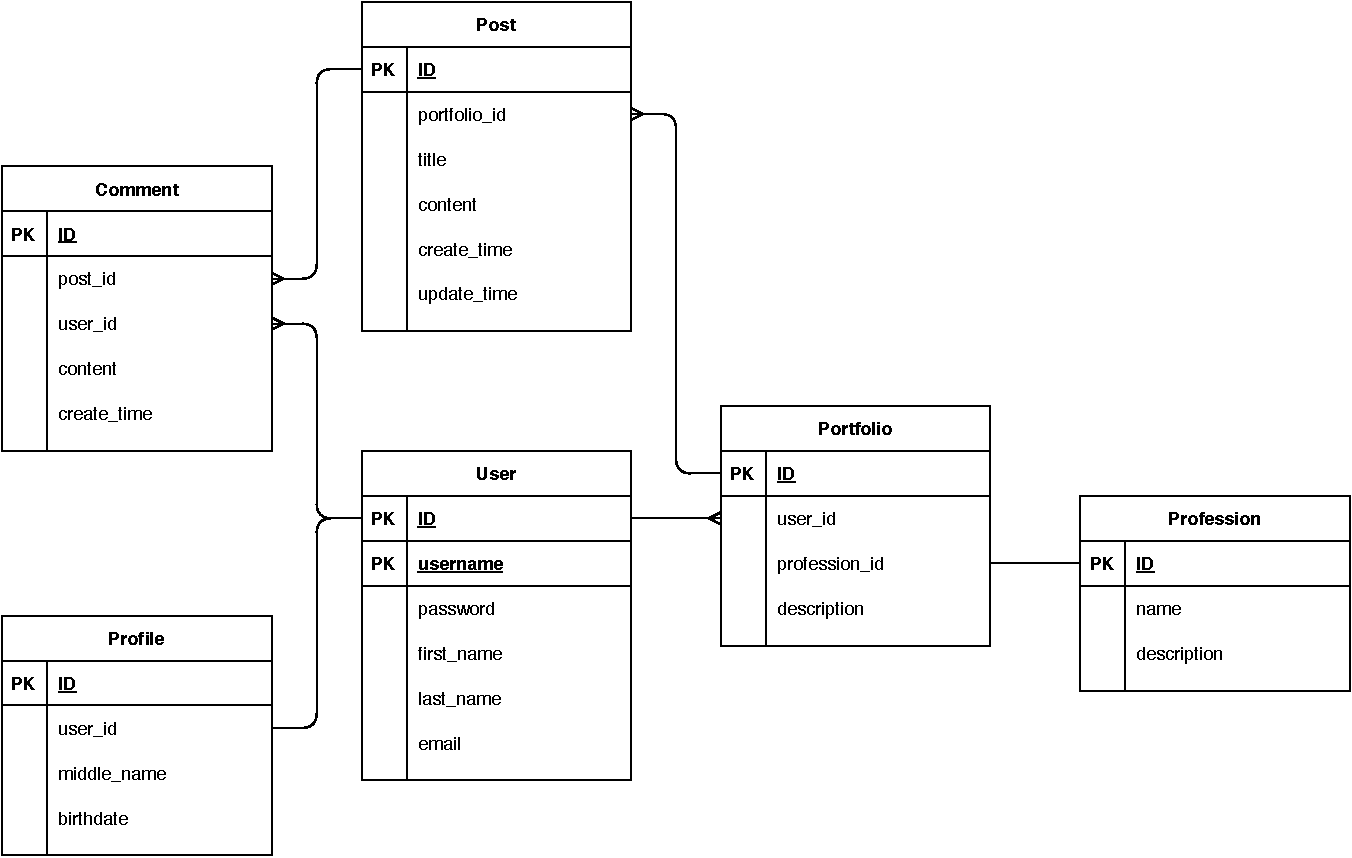
\includegraphics[scale=0.65]{pdf/er2.pdf}
    \caption{Обновлённая диаграмма Сущность-Связь}\label{img:er2}
\end{figure}

\subsection{Модели}%
\label{sub:modeli}

В листинге~\ref{lst:models} представлены модели Django данного проекта.

\begin{lstlisting}[caption={Модели Django}, label=lst:models]
from django.db import models
from django.contrib.auth.models import User

import datetime


class Profile(models.Model):
    user_id = models.ForeignKey(User, on_delete=models.CASCADE)
    middle_name = models.CharField('middle_name', max_length=30, null=True)
    birthdate = models.DateField('birthdate', null=True)

    def __str__(self):
        return 'Profile object (%d) of user (%d)' % (self.id,
                                                     self.user_id.id)


class Profession(models.Model):
    name = models.CharField('name', max_length=50)
    description = models.TextField('description')

    def __str__(self):
        return self.name


class Portfolio(models.Model):
    user_id = models.ForeignKey(User, on_delete=models.CASCADE)
    profession_id = models.ForeignKey(Profession, on_delete=models.CASCADE)
    description = models.TextField('description')

    def __str__(self):
        return '%s %s (%d) - %s' % (self.user_id.first_name,
                                    self.user_id.last_name,
                                    self.user_id.id,
                                    self.profession_id.name)


class Post(models.Model):
    portfolio_id = models.ForeignKey(Portfolio, on_delete=models.CASCADE)
    title = models.CharField('title', max_length=50)
    content = models.TextField('content')
    create_time = models.DateTimeField('create_time')
    update_time = models.DateTimeField('update_time', null=True)

    def __str__(self):
        return self.title


class Comment(models.Model):
    user_id = models.ForeignKey(User, on_delete=models.CASCADE)
    post_id = models.ForeignKey(Post, on_delete=models.CASCADE)
    content = models.TextField('content', max_length=140)
    create_time = models.DateTimeField('create_time')
\end{lstlisting}

\section{Описание интерфейса программы}%
\label{sec:opisanie_interfeisa_programmy}

Неавторизованному пользователю предоставляется возможность либо авторизоваться, либо пройти регистрацию учётной записи. На рисунке~\ref{img:scr_01} изображена форма регистрации, а на рисунке~\ref{img:scr_02}~--- форма авторизации.

\begin{figure}[H]
    \centering
    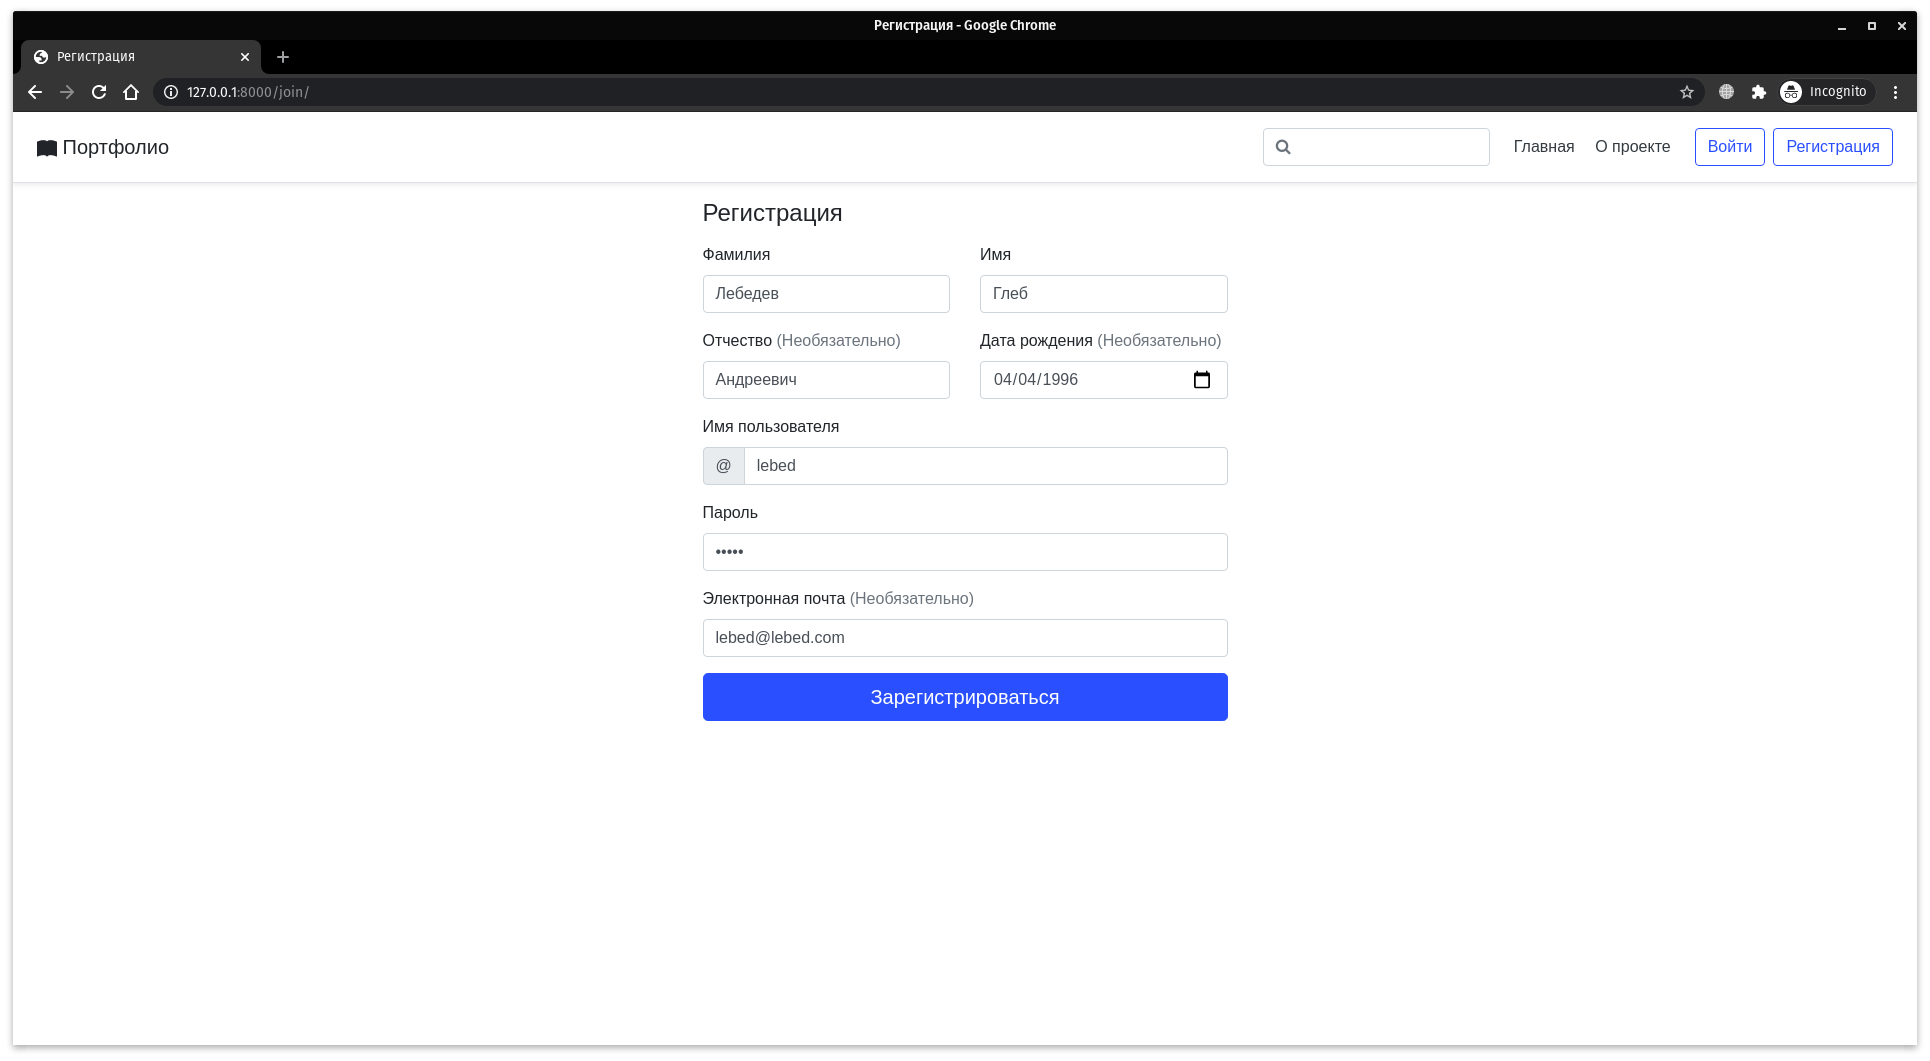
\includegraphics[scale=0.235]{images/scr_01.png}
    \caption{Форма регистрации}\label{img:scr_01}
\end{figure}

\begin{figure}[H]
    \centering
    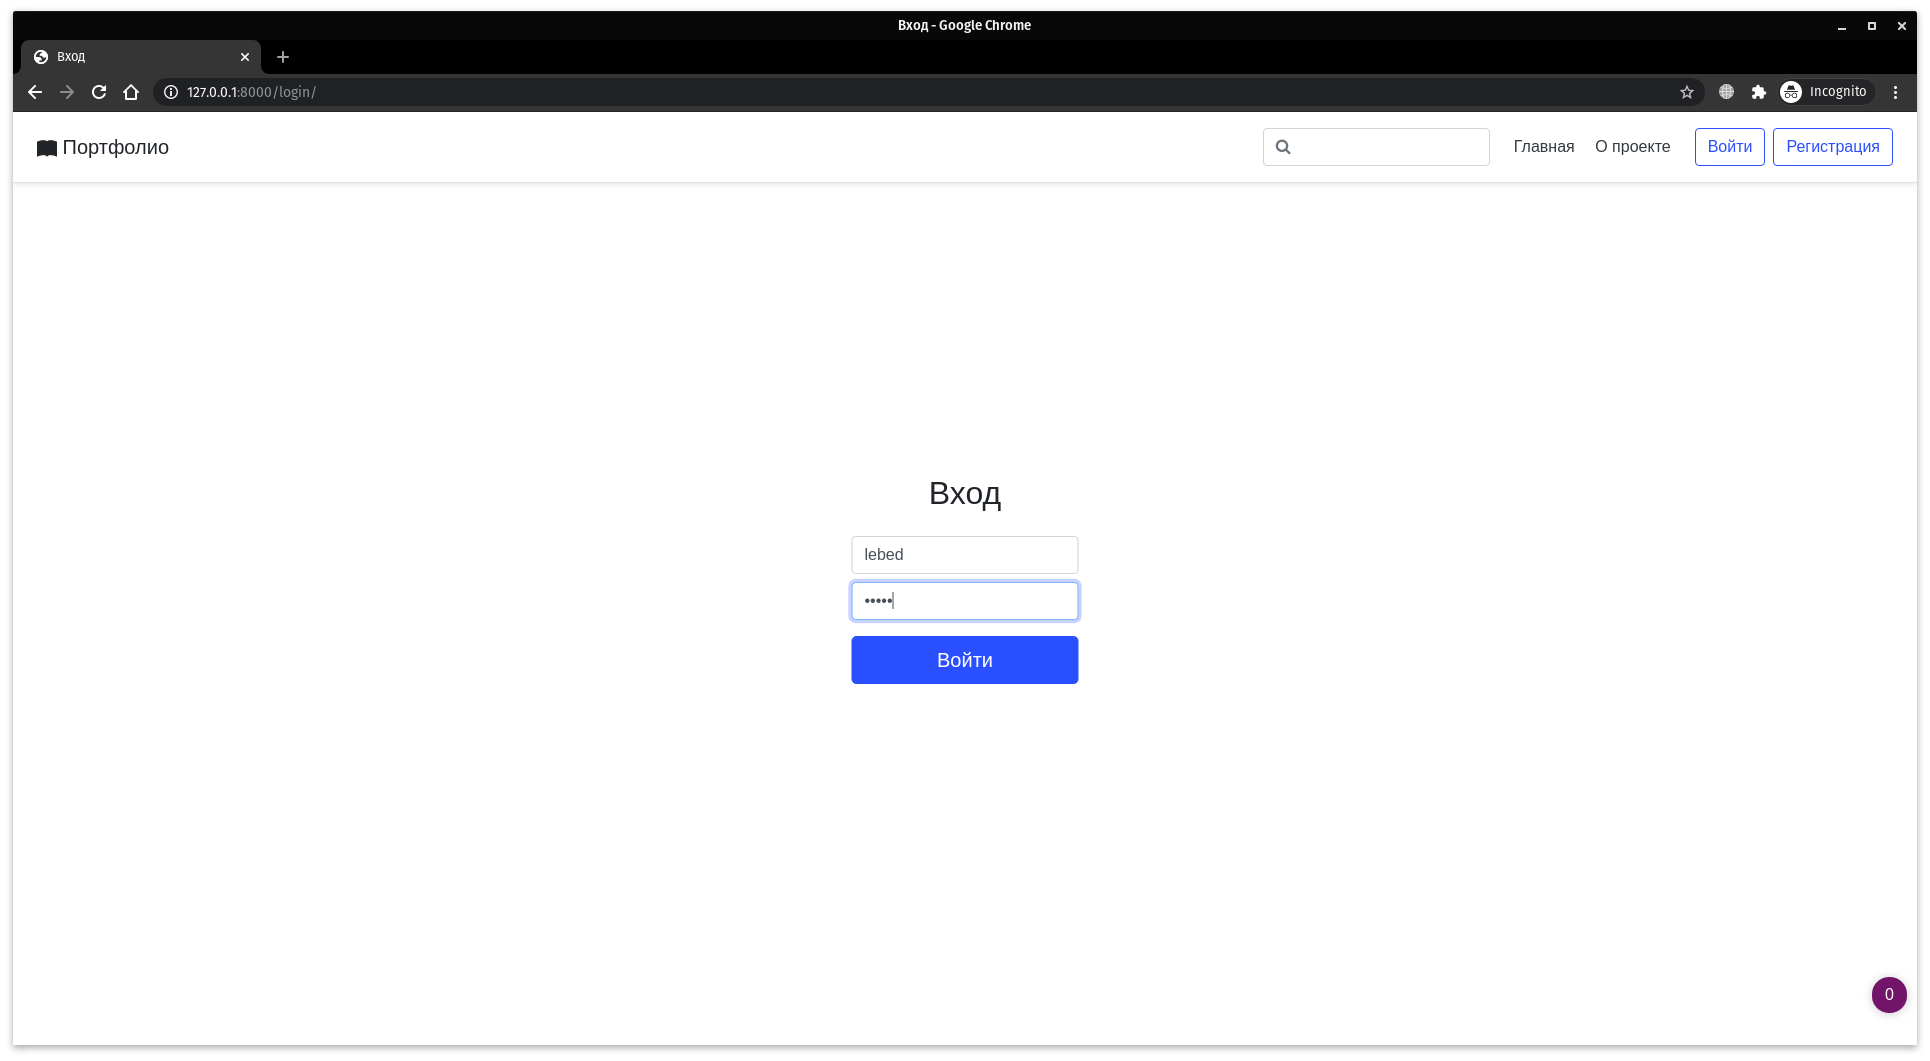
\includegraphics[scale=0.235]{images/scr_02.png}
    \caption{Форма авторизации}\label{img:scr_02}
\end{figure}

После авторизации пользователя приветствует его персональная страница, на которой отображаются информация о нём и список его портфолио. На рисунке~\ref{img:scr_03} изображена описанная страница пользователя. Кроме того, здесь пользователь может перейти к форме создания нового портфолио, нажав на соответствующую кнопку.

\begin{figure}[H]
    \centering
    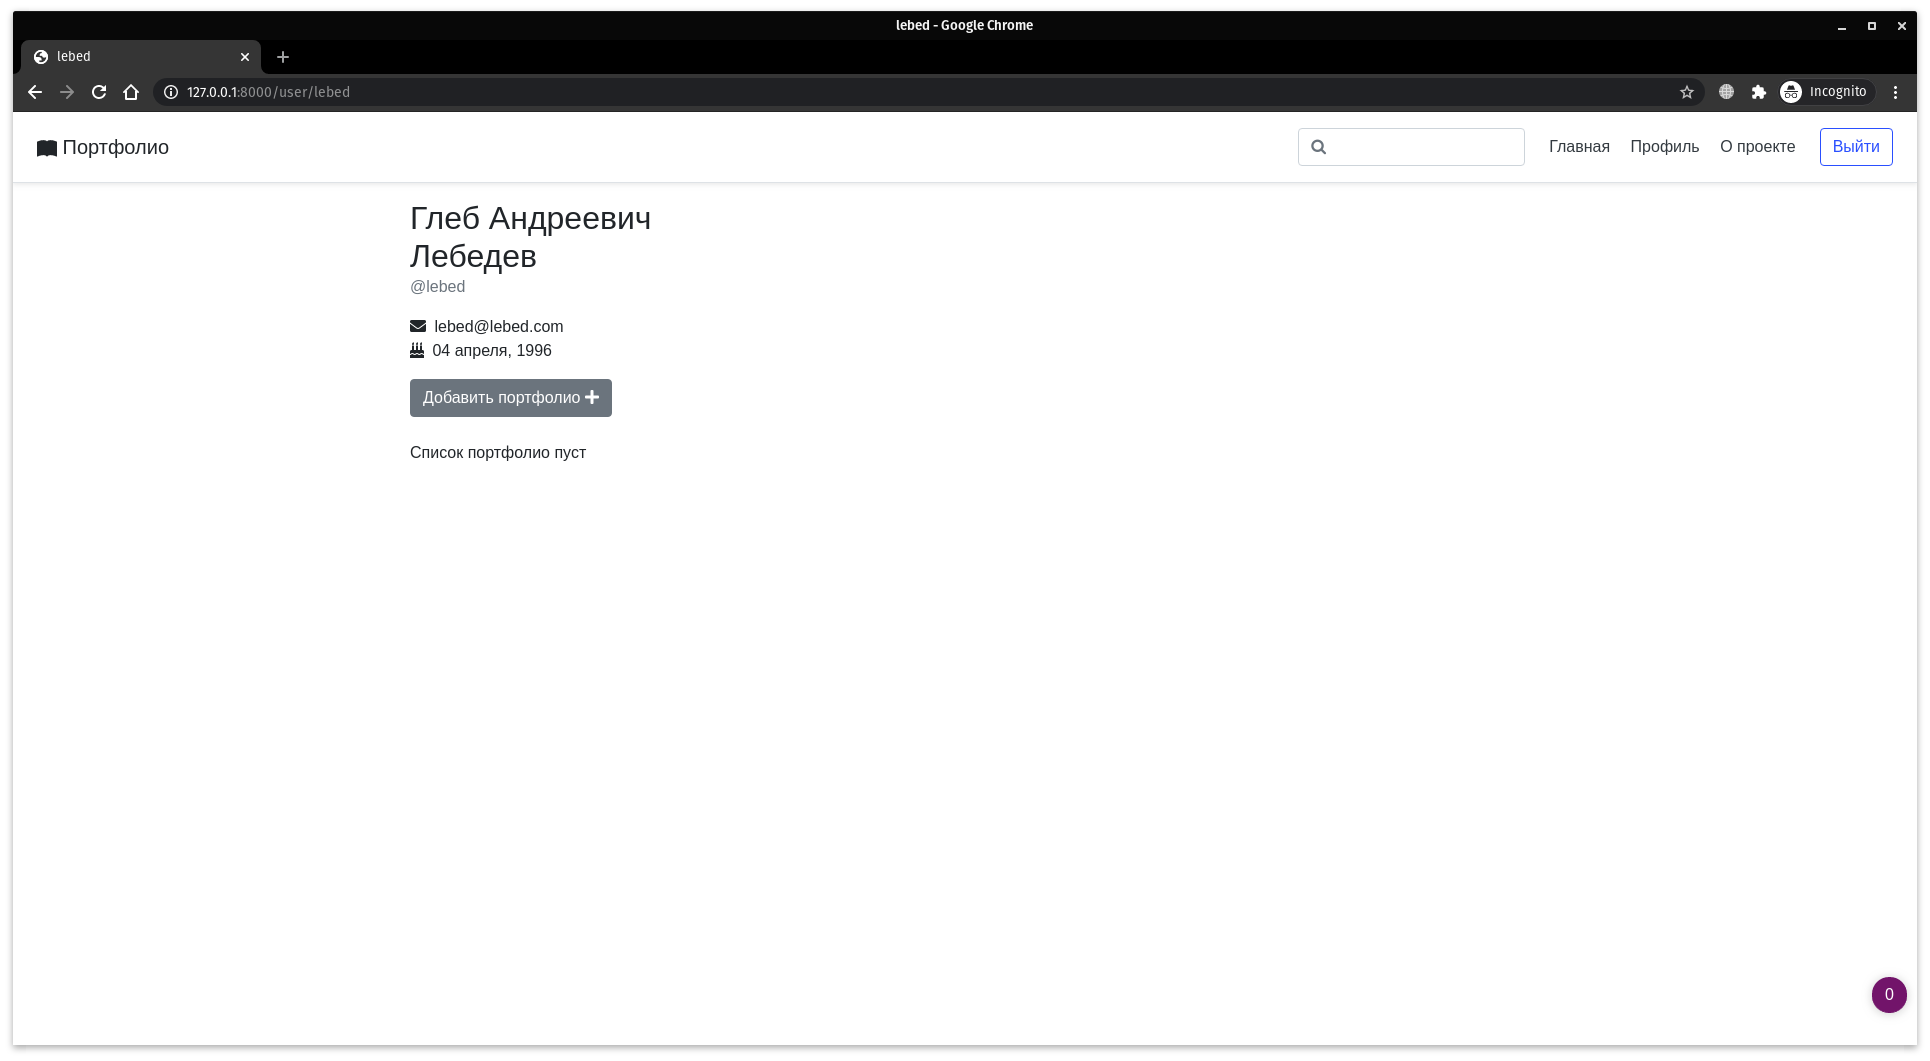
\includegraphics[scale=0.235]{images/scr_03.png}
    \caption{Персональная страница пользователя}\label{img:scr_03}
\end{figure}

На рисунке~\ref{img:scr_04} представлена форма создания нового портфолио. Данная форма доступна только авторизованным пользователям, остальные при попытке доступа к ней будут перенаправлены на форму авторизации.

\begin{figure}[H]
    \centering
    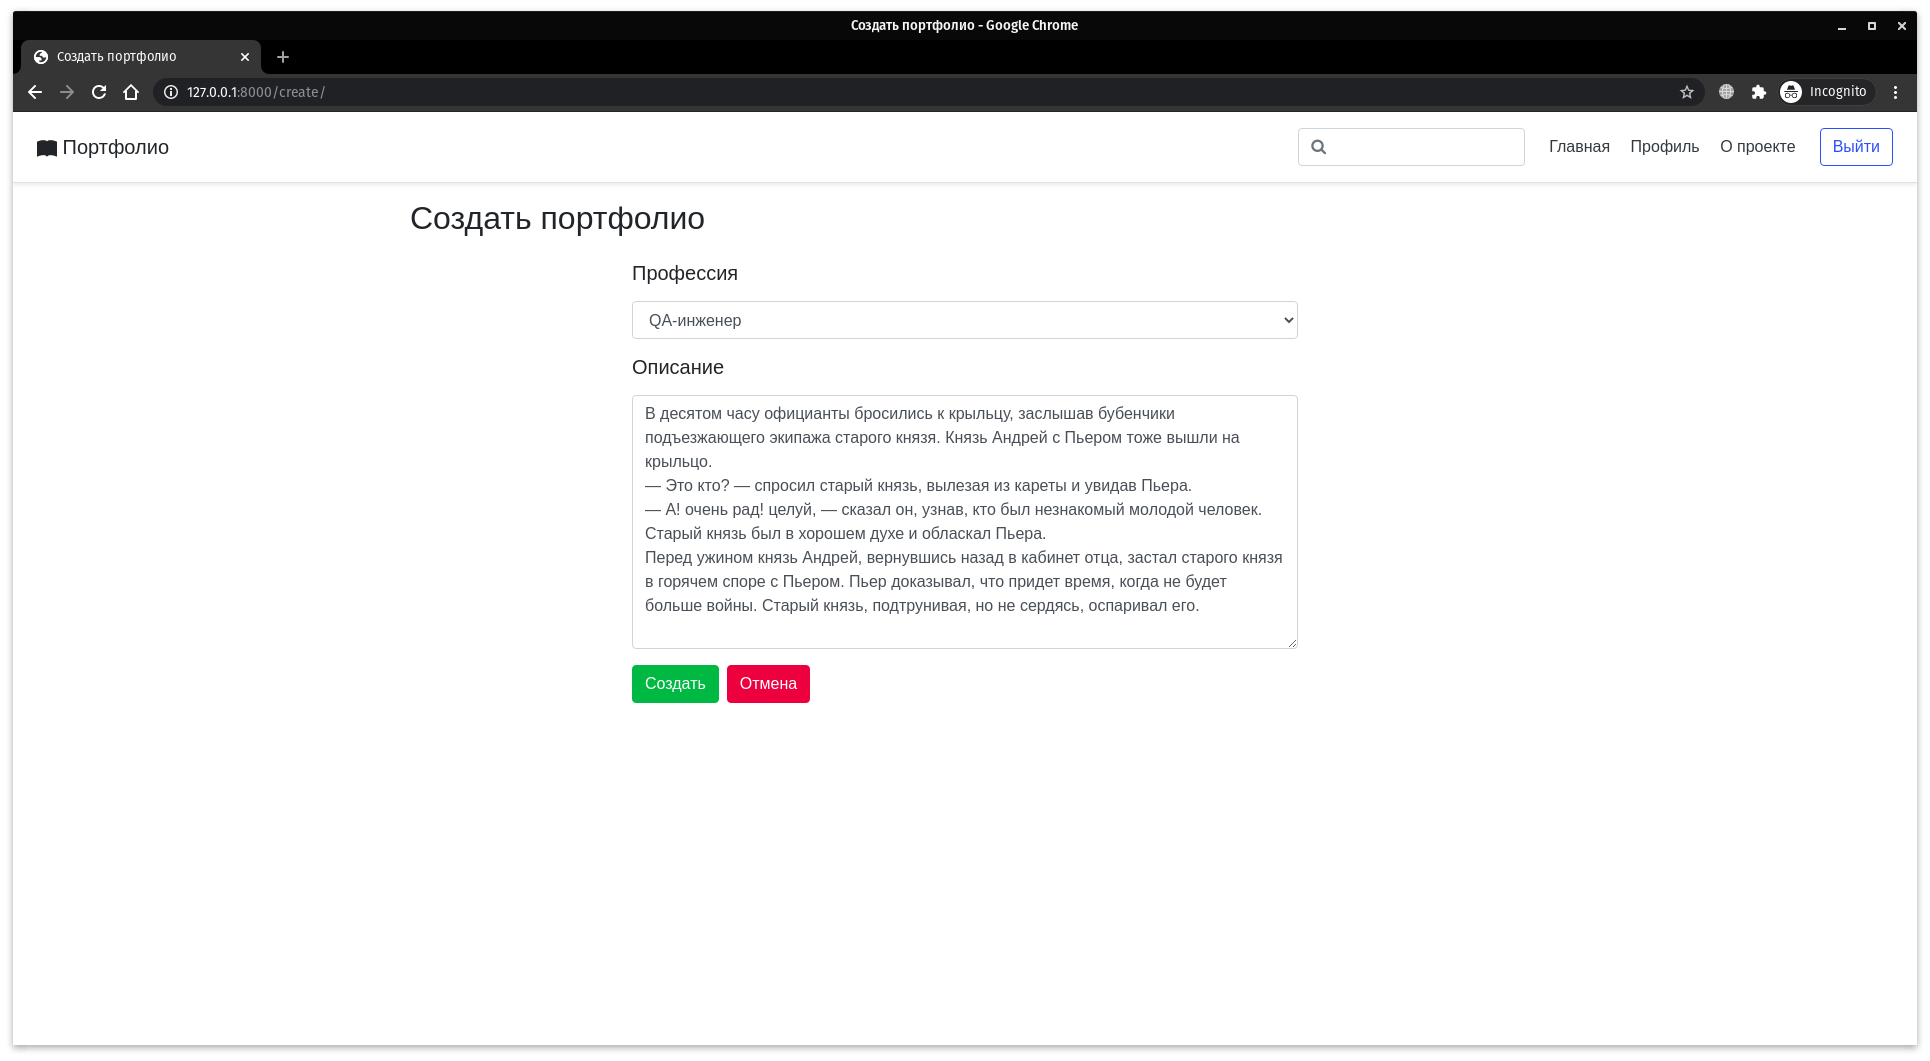
\includegraphics[scale=0.235]{images/scr_04.png}
    \caption{Форма создания нового портфолио}\label{img:scr_04}
\end{figure}

На рисунке~\ref{img:scr_05} изображена страница портфолио. Тут находятся указание пользователя-хозяина портфолио, указание и описание профессии для которой создано это портфолио, а так же список постов пользователя и форма для создания новых записей.

\begin{figure}[H]
    \centering
    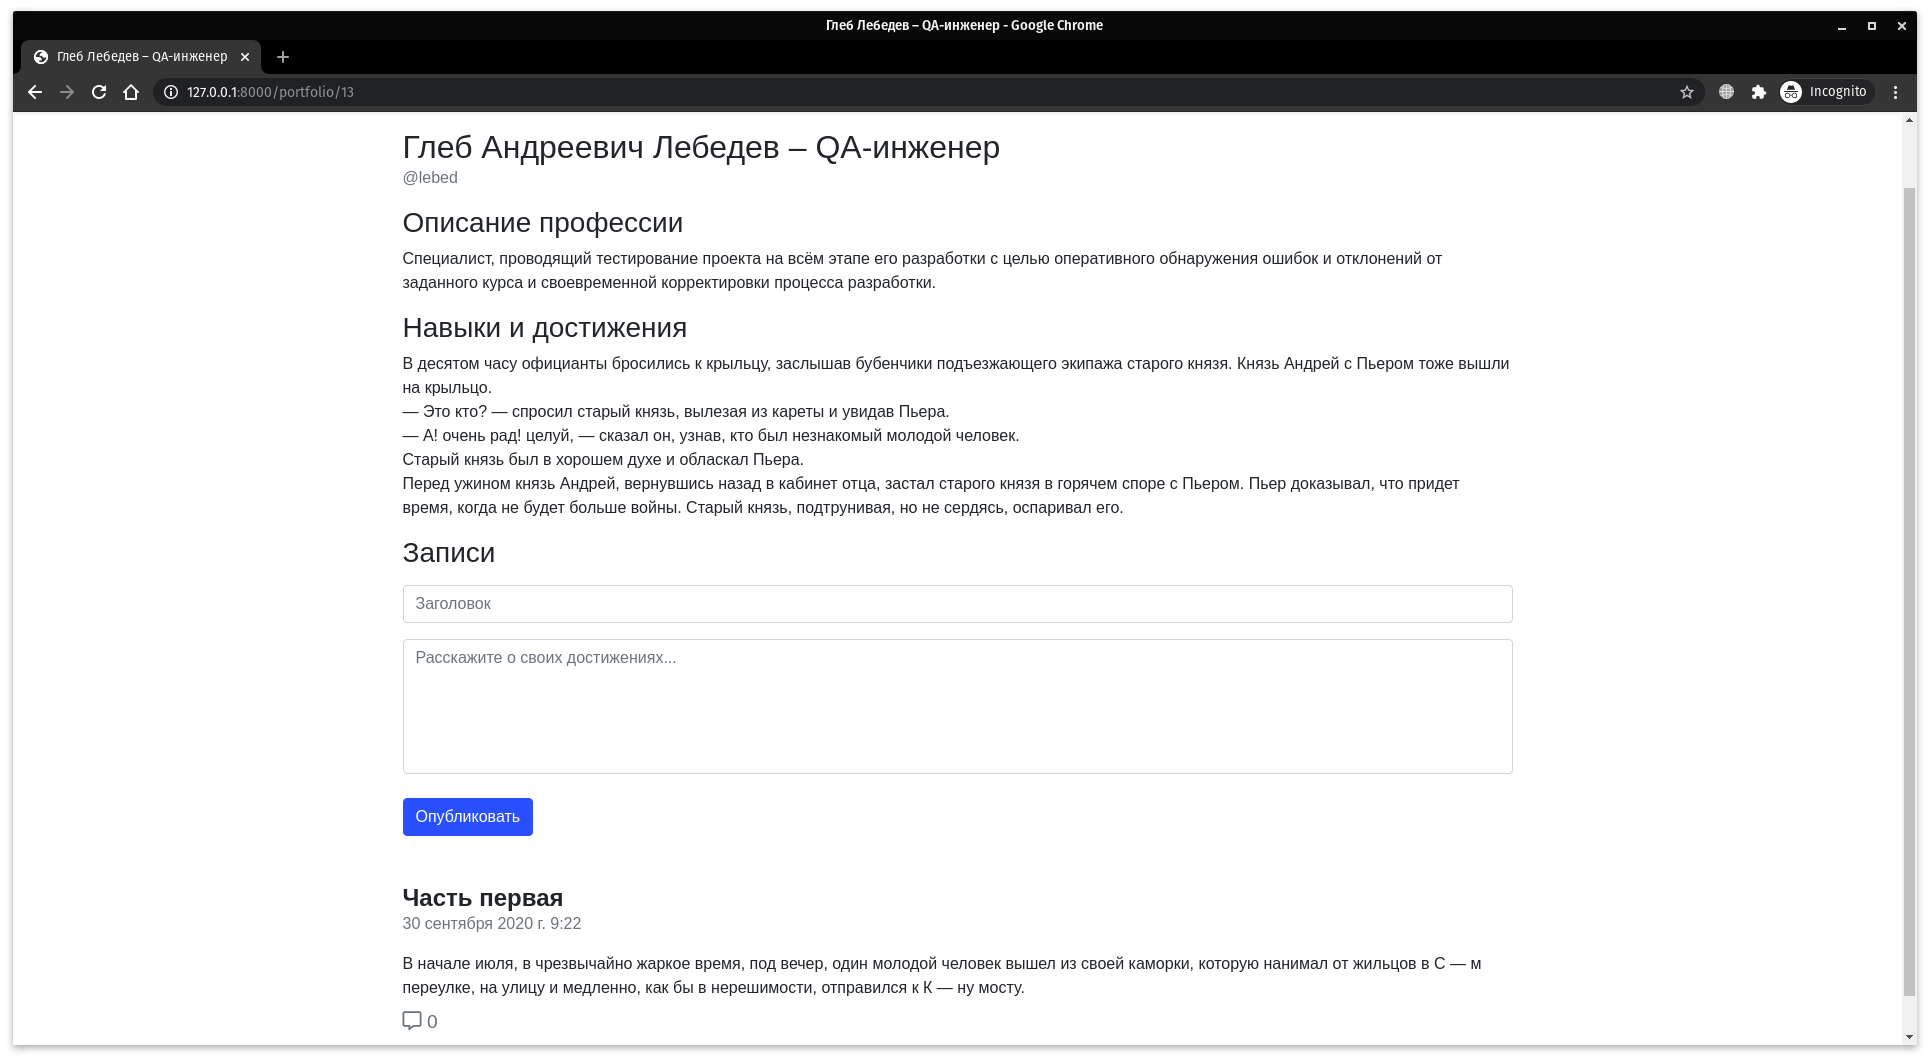
\includegraphics[scale=0.235]{images/scr_05.png}
    \caption{Страница портфолио}\label{img:scr_05}
\end{figure}

На странице записи (рисунок~\ref{img:scr_06}) помимо самой записи находится список комментариев пользователей и форма для создания нового комментария.

\begin{figure}[H]
    \centering
    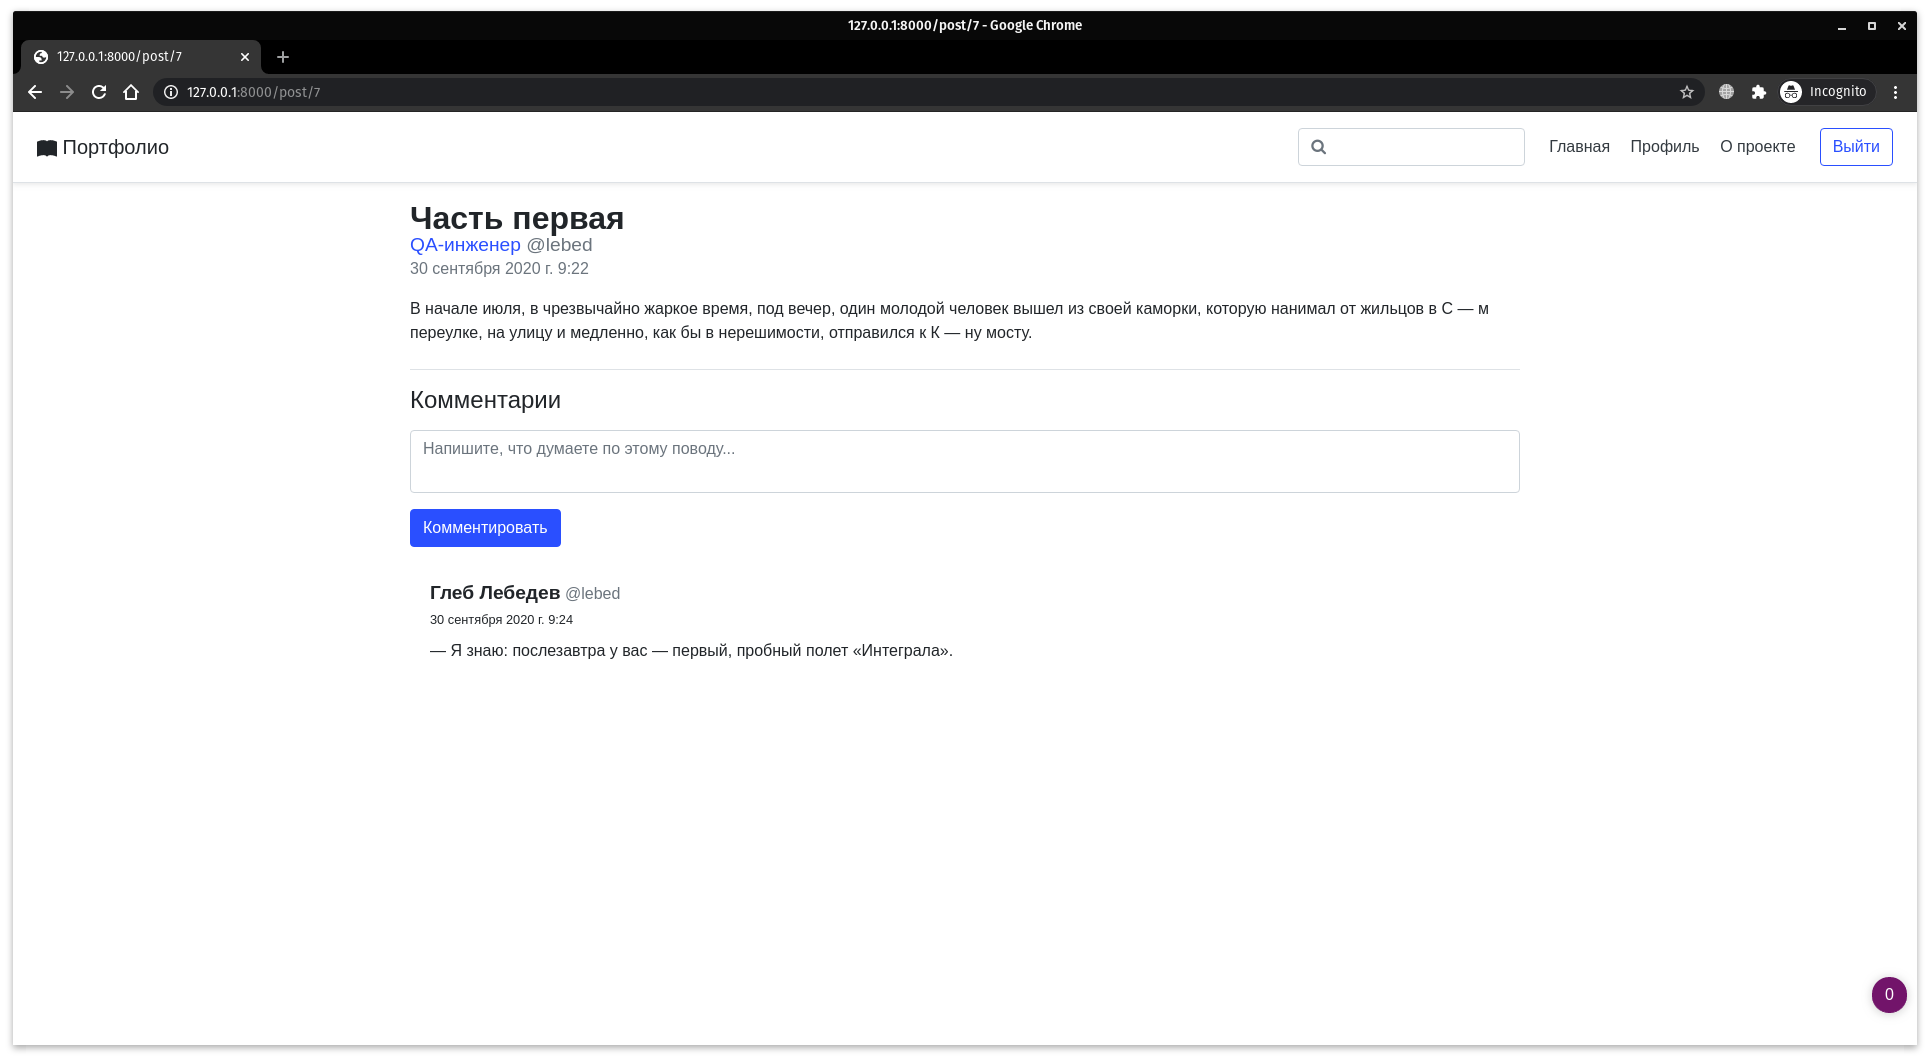
\includegraphics[scale=0.235]{images/scr_06.png}
    \caption{Страница записи}\label{img:scr_06}
\end{figure}

\section{Апробация}%
\label{sec:aprobatsiia}
Апробация проводилась на ноутбуке, подключённом к сети питания. Конфигурация ноутбука:
\begin{itemize}
    \item процессор Intel Core i5--8400H 2.5 ГГц;
    \item 8 гб ОЗУ;
    \item ОС Ubuntu 20.04.
\end{itemize}

Апробация показала работоспособность программы.

\section{Выводы}%
\label{sec:vyvody_impl}

В данном разделе был произведён выбор инструментов разработки и рассмотрены интерфейс web-приложения и его основыные функции.
